\section{Segmentation}
The process of segmentation is to separate the background to foreground.

\begin{itemize}
\item The Background subtraction use three parameters: \textbf{gamma},\textbf{tau} and \textbf{radius}.
	\begin{equation} Background_{i+1} = gamma*frame_{i} + (1-gamma)*Background_{i} \end{equation}
	\begin{itemize}
	\item Gamma is the learning rate, usually is 0,05.
	\item Tau is the different between frame to background.
	\item Radius is the parameter to delete the little blobs.
	\end{itemize}
	
\item The \textit{background subtraction} is not robustness to change illumination, for this we implement \textit{Grey-World} because is invariant to illuminant changes. 
The Grey-World method try to eliminate the grey in the image, for this reason move the minimum and the maximum values.

\begin{equation}
	( R' G' B' )= \left(
	\begin{array}{cccl}
		\frac{R_{grey}}{R_{m}(I)} & 0 & 0 \\
		0 & \frac{G_{grey}}{G_{m}(I)} & 0 \\
 		0 & 0 & \frac{B_{grey}}{B_{m}(I)}
	\end{array}
	\right) 
	* 
	\left(
	\begin{array}{c} R \\ G \\ B
	\end{array}
	\right)
\end{equation} 

\item The \textit{selectivity} is the other method that use the simple different between foreground with background but the selectivity a prior knows that pixel is or isn't foreground. 
	\begin{equation}
	\left \{
	\begin{array}{cccl}
		B_{i+1}(x,y) = \alpha * F_{t}(x,y)+(1-\alpha )* B_{t}(x,y) & if F_{t}(x,y) is Background \\
		B_{i+1}(x,y) = B_{t}(x,y) & if F_{t}(x,y) is Foreground
	\end{array} \right.
	\end{equation}


\item The \textit{eigenbackground} method use the Principal Component Analisys (PCA) to reduce the dimensionality. Also, the first M eigenvectors are the eigenbackground.
\begin{quote}
		eigenbackground = eigenvectors(:,1:M) \\
		Foreground = I - I' \\ 
		I' = Image Projection and Reconstruction (Background) \\
\end{quote}
\end{itemize}

\begin{figure}[h]
  \centering              
  \subfigure[Frame 300 - Background Subtraction]{
\includegraphics[width=0.3\textwidth]{frame300_segmented}}
  \subfigure[Frame 300 - Selectivity]{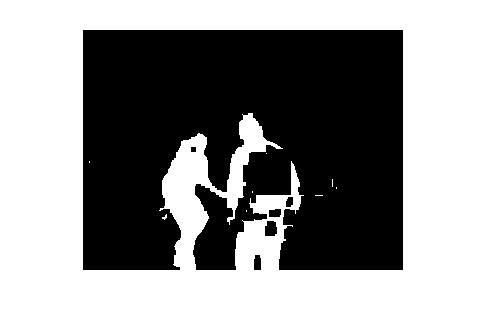
\includegraphics[width=0.3\textwidth]{frame300_selectivity}}
  \subfigure[Frame 300 - Eigenbackground]{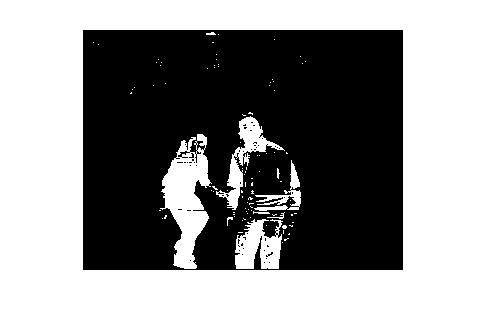
\includegraphics[width=0.3\textwidth]{frame300_eigenbackground}}
  \subfigure[Frame 300]{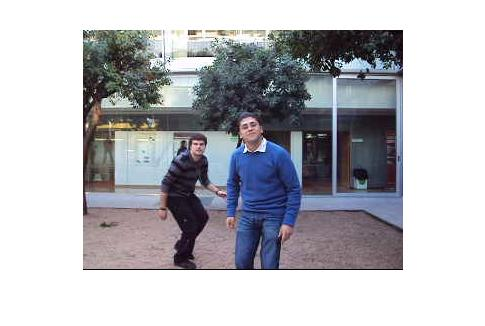
\includegraphics[width=0.3\textwidth]{frame300}}  
  \caption{Different segmentation with the same frame }
\end{figure}

